\documentclass[referee, 
		     sn-basic]{sn-jnl}

\usepackage{amssymb}
\usepackage{lineno}
\usepackage{booktabs}

\newcommand{\degC}{$^\circ$C}

% Springer stuff 
\jyear{2021}%
\raggedbottom
\unnumbered% uncomment this for unnumbered level heads

\begin{document}
\raggedright

\title[Weather, fuel, and grassland fire behavior]{Weather and fuel as modulators of grassland fire behavior in the northern Great Plains}

\author*[1]{\fnm{Devan Allen}  \sur{McGranahan}}\email{Devan.McGranahan@usda.gov}
\author[2]{\fnm{Megan E.} \sur{ Zopfi}}\email{Megan.Zopfi@und.edu }
\author[2]{\fnm{Kathryn A.} \sur{ Yurkonis}}\email{Kathryn.Yurkonis@und.edu}

\affil[1]{\orgname{USDA Agricultural Research Service}, 
	     \orgdiv{Livestock \& Range Research Laboratory},
              \orgaddress{\street{243 Ft. Keogh Rd.}, 
            		     \city{Miles City},
            		     \postcode{59301}, 
           		     \state{Montana},
            		     \country{USA}}}
\affil[2]{\orgname{University of North Dakota}, 
            \orgdiv{Department of Biology},
            \orgaddress{\street{10 Cornell St.}, 
            		   \city{Grand Forks},
            		   \postcode{58202}, 
           		   \state{North Dakota},
            		   \country{USA}}}


\abstract{Fuel and weather interact to affect wildland fire behavior, but little is known about associations between these variables
in the northern Great Plains of North America. Few studies consider rate of spread or statistically test the influence of fuel and weather.
We measured overall fuel load and moisture ahead of prescribed fires in North Dakota, USA, and used a thermocouple array to
measure two-dimensional rate of spread, soil surface temperature, and aboveground flame temperature, to compare with fire weather data.
Flame temperatures averaged 225\degC~during spring burns and 250\degC~during fall burns, and were generally higher with greater fuel loads and lower overall fuelbed moisture.
Surface temperatures averaged $\approx$100\degC, although 50\% of observations were $\leq$60\degC. 
Fires spread at an average of 2.5 m min\textsuperscript{-1}, increasing with wind speed.
As such, prescribed fire in northern Great Plains working rangeland appear to spread slowly and effect low soil surface temperatures, often limited by high fuelbed moisture. 
Fire behavior measurements respond differently to variability in fuel and weather. 
Belowground heating is likely minimal.
We suggest ecologists ought to consider which fire behavior measurements best relate to fire effects, and managers consider weather and ignition pattern mitigations when fuels constrain desired fire behavior to ensure effective burns.}

\keywords{Grassland fire ecology and management, Prescribed fire, Rangeland fire management, Robust wildland fire science, Wildland fire science in working landscapes} 

\maketitle
\begin{linenumbers}

\hypertarget{introduction}{%
\section{Introduction}\label{introduction}}

Prescribed fire is used widely for ecosystem management around the world \citep{weir2022}. 
More than simply the result of combustion of vegetation, wildland fire behavior is multi-faceted, with different components producing different effects on the surrounding environment and organisms within. 
Most wildland fire scientists describe fire behavior in terms of \emph{rate of spread}---how quickly a flame front moves through a fuelbed---and \emph{intensity}---a suite of measurements of how much energy is released by combustion, often expressed as a rate of energy release over time \citep{mcgranahan2021a}.

Wildland fire behavior is controlled by interactions among several
abiotic and biotic factors, and understanding them is critical to safe
and effective wildland fire management \citep{benson2009}. \emph{Abiotic
factors} include those determined by the physical environment, such as
wind speed and atmospheric moisture content. Wind speed has long been
recognized as a primary driver of fire behavior, especially in
well-cured grassland fuels
\citep{whittaker1961, cheney1995, kidnie2015}. Two measures of
atmospheric moisture content---relative humidity and vapor pressure
deficit---are also associated with fire growth
\citep{evett2008, reid2010, sedano2014}.

\emph{Biotic factors} relate principally to the amount and nature of
plant biomass available for combustion. Overall, energy release rates
increase as more fuel is available to burn. The structure and
arrangement of vegetation is also important. Greater fuel load
attributable to longer time-since-fire increases fire temperature, and
spatial variability in fuel load and patchy distribution of fine fuels
in turn drive variability in fire behavior
\citep{patten1984, gibson1990, gomes2020}. Furthermore, fine-leaved
grasses burn more completely and hotter than an equal mass of forbs
\citep{wragg2018}. Finally, fuel moisture content is an especially
important driver outside of the highly-cured context of wildfire seasons
\citep{sparling1966, kidnie2015}. Together, variability in flammability
traits and curing rates among species that comprise grassland fuelbeds
contributes to variability in fire behavior
\citep{cruz2015, kidnie2015, mcgranahan2016, cardoso2018}.

How and where within the wildland fire environment fire behavior
measurements are made matters a great deal to assessing fire effects.
For decades, fire ecologists have measured fire behavior as \emph{flame
temperature} via various methods, including arrays of
temperature-sensitive paints
\citep[e.g.,][]{whittaker1961, smith1966, bailey1980} or by recording
air temperature as a flame front passes over a thermocouple connected to
a datalogger \citep[e.g.,][]{strong2013, russell2015}.

Despite its popularity among fire ecologists, temperature alone is a
poor response variable fraught by several issues in collecting and
interpreting thermocouple data \citep[see review by][]{mcgranahan2020}.
Firstly, a considerable amount of variability in temperature is
attributable to sensor placement relative to both the ground and the
fire. There is neither a standard for placing thermocouple probes in the
wildland fire environment nor consistency in vertical temperature
profiles. Most observations of surface fire temperature profiles
describe an inverse, linear relationship between height and temperature
\citep{smith1966, patten1984, archibold2003}, although
\citet{ramsay1996} found the highest temperatures at the top of a 1 m
profile and the lowest temperatures at 30 cm, while \citet{frost1987}
and \citet{bailey1980} present evidence that the highest temperatures
occur midway up the profile. At least some of this variability might be
due to differences in surface vs.~flame temperature among head and back
fires \citep{trollope1978}.

Secondly, many factors that contribute to variability in temperatures
recorded by thermocouples are attributable to the nature of the sensor
rather than the nature of the fire \citep[e.g.,][]{walker1968}. Thus,
reporting `device temperatures' alone impedes comparisons between
studies; \citet{bova2008} present a standard calibration of thermocouple
probes, while \citet{mcgranahan2021b} simply uses the timestamps of peak
heating across an array of several thermocouples to calculate rate of
spread. Using rate of spread as the response variable makes moot the
third issue with temperature as a fire behavior metric: temperature of
the media around a probe is a poor proxy for the thermal experience of
an organism. Measures of intensity or energy flux are more biologically
relevant \citep{kremens2012, smith2016}.

In the North American Great Plains, most reports of grassland fire
behavior consist of temperatures derived from thermocouples, and there
are few data on rate of spread. Soil surface temperatures in South
Dakota tallgrass prairie ranged from 200-500\(^\circ\)C during spring
burns, and were greatest under lower fuel loads \citep{ohrtman2015};
fires in Saskatchewan mixed grass prairie exceeded 300\(^\circ\)C 5-10
cm above the soil surface in spring, summer, and fall
\citep{archibold2003}. Mean temperatures in experimental burns in
eastern Montana ranged from 172-222\(^\circ\)C in the summer to 253\(^\circ\)C in the spring \citep{strong2013, russell2015}. To our
knowledge, no studies on grassland fire in the northern Great Plains
region has explicitly tested the effect of fire weather on fire
behavior.

Our objectives were to (1) describe the range of variability in three
measures of fire behavior---rate of spread, soil surface temperature,
and flame temperature 15 cm above soil surface---during prescribed burns
in typical fuelbeds of the northern US Great Plains, and (2) explain
variability in fire behavior in terms of abiotic and biotic factors.
Our analysis emphasizes the differential effects of environmental variables among the three measures of fire behavior, and the multidimensional relationship among these responses during prescribed burns conducted at scales consistent with land management in the region.

\hypertarget{methods}{%
\section{Methods}\label{methods}}

\hypertarget{study-locations}{%
\subsection{Study locations}\label{study-locations}}

We sampled 25 prescribed fires at two locations in central and
southwestern North Dakota, USA (Maps in Supplemental Information Figure
1). At both locations, sampled grasslands are included in a patch-burn
grazing study that requires a portion of each experimental unit to be
burned each year \citep{spiess2020}. The majority of the burn units were
16 ha, while a small set were 8 ha. Typical ignition patterns consisted
of downwind backing fires followed by either ring ignition and primarily
head fire spread, when fuels were conducive; when fuels were sparse or
higher-moisture, flanking fires and strip ignitions were employed as
necessary to ensure fire spread through the entire burn unit.

In central North Dakota, we sampled 15 spring (May) fires at the North
Dakota State University Central Grassland Research Extension Center near
Streeter, ND (46.718686 N, 99.448521 W). Burned grasslands at this
location are divided into two 260 ha blocks with four, 65 ha pastures
each in which either an 8- or 16-ha patch is burned each spring. Located
in a mixed-grass prairie ecoregion, this location has a rolling
topography and receives an average of 468 mm annual precipitation.
Vegetation is mixed-grass prairie invaded by introduced, C\(_3\)
grasses; stands are dominated by \emph{Pascopyrum smithii},
\emph{Nassella viridula}, \emph{Poa pratensis}, \emph{Bromus inermis},
\emph{Koeleria macrantha}, \emph{Artemisia} spp., \emph{Solidago} spp.,
and clumps of \emph{Glycyrrhiza lepidota} and \emph{Symphoricarpos
occidentalis}.

In southwestern North Dakota, we sampled ten, 16-ha fall (October) fires
in two blocks at the North Dakota State University Hettinger Research
Extension Center, Hettinger, ND (46.004443 N, 100.646477 W) with mean
annual precipitation of 380 mm. Topography is consistently flat. Located
in a shortgrass prairie ecoregion, these pastures are dominated by
introduced C\(_3\) grasses \emph{Thinopyrum intermedium}, \emph{Bromus
inermis}, \emph{Agropyron cristatum}, and \emph{Poa pratensis}, along
with the non-native legume \emph{Medicago sativa}.

\hypertarget{data-collection}{%
\subsection{Data collection}\label{data-collection}}

We measured each fire with a set of 9, 1-m equilateral triangle plots
arranged in a nested fashion such that three 10 m triangles, each
containing 3, 1-m plots, were placed 100 m apart to form a total plot
area of 0.433 ha with 27 sample points positioned at the centroid of
each burn unit (a schematic of this layout is presented in Supplemental
Information Figure 2). This fractal design is modified from the
Sierpinksi triangle described by \citet{dorrough2007} and applied to
measuring wildland fire spread by \citet{mcgranahan2021b}. Although the
logarithmically-scaled nested design was intended for geospatial
analysis of point-level data, for our analyses here we calculate
averages from the finest (1 m microplot) scale, consistent with the
method of locating multiple microplots within larger burned areas to
characterize spatial variability within fires \citep{fernandes2000}.

\textbf{Fuel data} were collected no more than three hours prior to fire
ignition. We clipped and collected all fuels in a 25 × 25 cm quadrat
positioned 0.5 m away from each 1 m triangle vertex; the three
measurements per plot were averaged prior to analysis. Fuel samples were
initially placed in airtight plastic bags to retain moisture, and then
weighed, dried to constant mass at 60\(^\circ\)C for 48 hours, and
reweighed. These data were used to calculate percent fuel moisture
content (expressed on a dry-weight basis) and fuel load (kg m\(^{2}\))
for each plot (n = 9 subsamples for each fire).

\textbf{Fire behavior data} were recorded as temperature (\(^\circ\)C) associated with the advancing flame front at each of the 27 points arranged in 9, 1-m triangular microplots at the center of each burn
unit. Data were recorded with the open-source FeatherFlame thermocouple
datalogger system \citep{mcgranahan2021b}, logging at 1.5 Hz. The
FeatherFlame system reads overbraided, ceramic fiber-insulated, 20-gauge
K-type thermocouples (Omega, Norwalk, CT) connected to an Arduino-based
datalogger assembled from Adafruit Feather breakout boards (M0
Adalogger, datalogging shield, and OLED display; Adafruit Industries,
LLC, New York City, NY) and housed inside water-resistant Pelican cases
(Pelican Products, Inc, Torrance, California). 
The low cost of open-source systems make multiple units more affordable than proprietary data loggers with no sacrifice in data quality \citep{mcgranahan2021}.
More details on the datalogger system are available in Supplemental Information.

Another advantage of the multi-channel datalogger is the opportunity to calculate \emph{two-dimensional rate of spread} from the arrival time of the flame front at vertices of a thermocouple array logged to a common timestamp. 
While one-dimensional rate of spread requires direct observation of a flame front moving perpendicular to a vector of fixed points, two-dimensional rate of spread is ideal for larger-scale fires in which direct observation is infeasible and the exact angle of approach for oncoming flame fronts is not known \citep{finney2021}. 
Here, we calculate 2-D rate of spread through the 1 m triangular microplots using trigonometric equations from \citet{simard1984}.

At each 1 m triangular microplot---the observational unit in the nested plot design---we used four thermocouples connected to a single FeatherFlame datalogger. 
Three thermocouples measured flame temperature 15 cm above the soil surface at each 1 m vertex while a fourth thermocouple recorded soil surface temperature at a representative point within the 1 m array. 
Beads of the thermocouple probes extended at least 3 cm from the supporting apparatus, to which the insulated lead was attached with wire. 
The soil thermocouple was placed on mineral ground, perpendicular to the soil surface, below plant litter.

For each fire event, we determined the time and value of the maximum temperature (\degC) as the flame front encountered each thermocouple. 
We calculated the maximum flame temperature (\degC) 15 cm above soil surface for each microplot as the mean of the thermocouple readings from its 3 vertices. 
We calculated the rate of spread (m min\textsuperscript{-1}) of the flame front as it passed through
each microplot using the maximum temperature timestamps as arrival times following equations from \citet{simard1984}, which are presented in full in Supplemental Information.

\textbf{Fire weather data} were obtained after each fire from records
made available by the North Dakota Agriculture Weather Network, the
statewide mesonet system with sensor arrays at both experimental
stations. We downloaded hourly relative humidity (\%), dew point
(\degC), air temperature (\degC), and average wind speed (m s\textsuperscript{-1}). From these data we calculated atmospheric vapor pressure ($e$) and saturation vapor pressure ($e_s$) and used these
quantities to determine the vapor pressure deficit ($VPD = e - e_s$)
for the hour in which each fire behavior observation occurred. These
data capture hourly trends in weather at the meso-gamma scale \citep[2-20 km;][]{orlanski1975}, and are reliably connected to our fire behavior measurements via time stamps provided by the dataloggers. 
The Hettinger mesonet array is 3--8 km from burned pastures, while the Central Grasslands mesonet array is 1--7.5 km from burned pastures. We
found a high degree of consistency between these meso-scale data and
fire weather records made on the fireline during operational periods,
and the open rangeland physiognomy with flat to rolling terrain
precludes substantial microsite differences in weather between these
records and the conditions at each fire behavior sample point.

\hypertarget{data-analysis}{%
\subsection{Data analysis}\label{data-analysis}}

Prior to analysis, we ensured statistical power across 167 observational
units by using multiple imputation to interpolate missing datapoints, as
missing field data occurred for three rate of spread samples (2\% of
total), 29 fuel load values (17\%), and 46 soil surface temperature
values (27\%) due to logistical and time constraints during the
operational burn periods. We used the multiple imputation method in the
\emph{mice} package \citep{vanbuuren2011} in the \textsf{R} statistical environment \citep{rct2020} to fill in these missing values. 
The procedure simulated 50 datasets with different, but reasonable, values for the missing data based on patterns in the existing data. 
We then scaled all variables to a common range within each imputed dataset, performed regression analysis on each \emph{mice}-generated dataset, and report composite statistical results pooled from the results of the 50 individual regression models.

\textbf{Multivariate analysis.---}We first conducted a multivariate analysis to assess composite relationships among the fuel, weather, and fire behavior responses. 
We used Principal Components Analysis (PCA) fit with the \texttt{rda} function in the \emph{vegan} package for \textsf{R} \citep{oksanen2017}. 
We performed post-hoc group (location) and gradient (fire weather) analysis with the \emph{vegan} \texttt{envfit} function, stratified by year.

\textbf{Regression analysis.---}We assessed weather and fuel effects on three fire behavior response variables: Maximum flame temperature (\degC) 15 cm above the soil surface (mean of three thermocouples), maximum soil surface temperature (\degC; single thermocouple), and rate of spread (m min\textsuperscript{-1}) through each 1 m triangular microplot. 
Because all three response variables were best modeled with a gamma distribution, we fit generalized linear mixed-effect regression models for each response with the \texttt{glmer} function from the \emph{lme4} package in \textsf{R} \citep{bates2015}. 
Fixed effects consisted of weather and fuel variables, as described above. 
The
random-effect term was constructed to account for random variance among
locations, spatial non-independence within locations and nested variance
within sample plots, and the effect of repeated measurements within each
location. Due to concerns about collinearity between relative humidity
and vapor pressure deficit because they are derived from the same
variables, vapor pressure deficit was excluded from regression analysis
for all three response variables.

\hypertarget{results}{%
\section{Results}\label{results}}

\begin{figure}[!h]
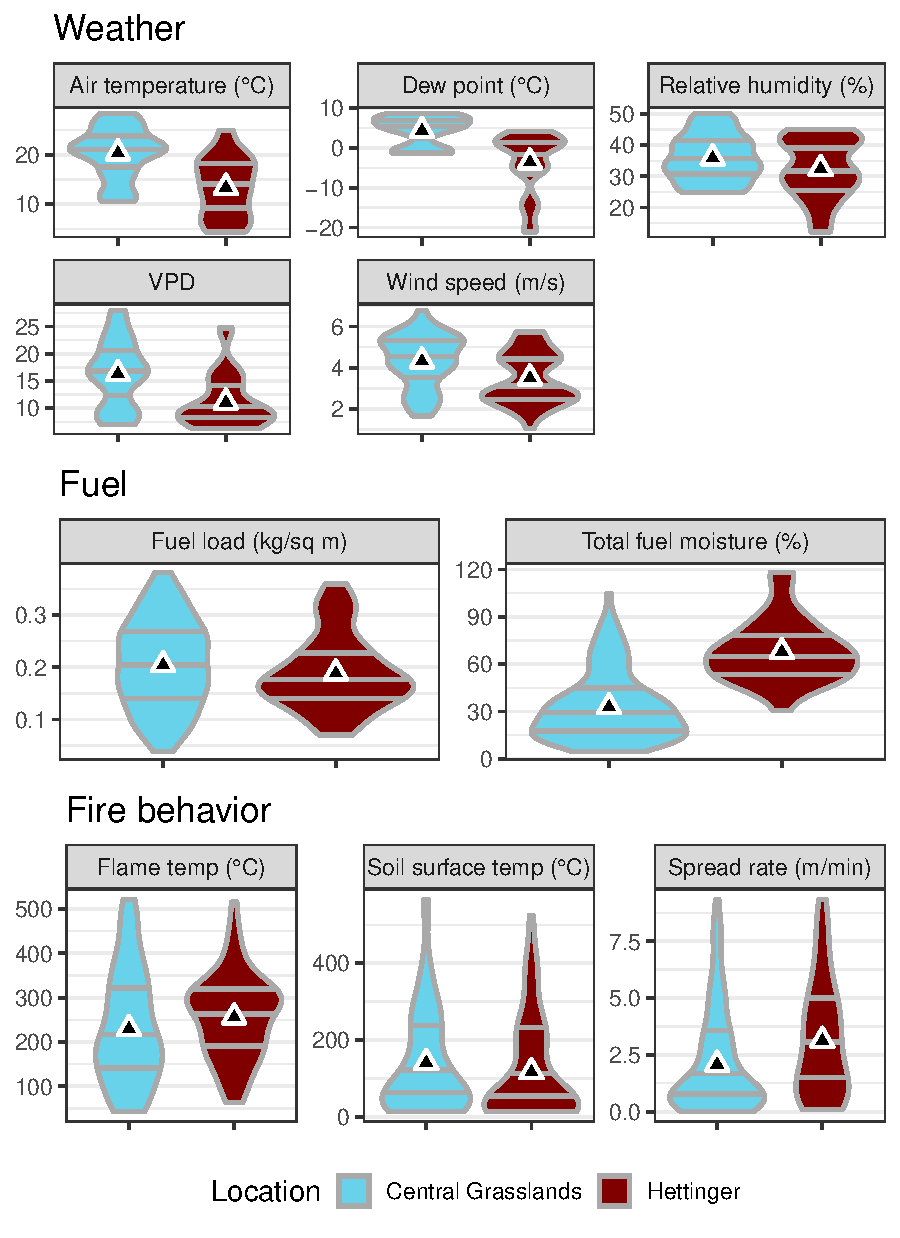
\includegraphics[width = 1\columnwidth]{data_summary_gg-1.pdf}
\caption{Distribution of weather, fuel, and fire behavior data for fires in southwestern North Dakota (Hettinger, dark maroon) and central North Dakota (Central Grasslands, light blue). 
Horizontal gray lines denote 25\%, 50\% (median) and 75\% quantiles; triangles are arithmetic means. 
Means and standard deviation are also reported in Supplemental Information Table 1. 
VPD = Vapor pressure deficit.}
\label{DataSummary}
\end{figure}

Most measures of fuel, fire weather, and fire behavior showed
considerable variability within each location, although rates of spread
were generally low (Fig.~\ref{DataSummary}). 
Principal Components Analysis indicated fire behavior patterns were consistent across locations ($P$ = 0.11), although the fall season in Hettinger---our semi-arid location in southwestern North Dakota---tended to have drier air and hotter fires (Fig.~\ref{PCA}). 
Spring fires in the Central Grasslands were conducted under warmer and more evaporative (VPD) conditions than fall fires at
Hettinger. The first two axes of the Principal Components Analysis (Fig.
2) explained 86\% of overall variance in the fire behavior dataset. The
first axis (52\% variance explained) was most strongly associated with
flame temperature and rate of spread, while the second axis was more
strongly associated with soil surface temperature. Dew point was
marginally related ($P~<$ 0.05) and inversely associated with
flame temperatures and rate of spread.

\begin{figure} 
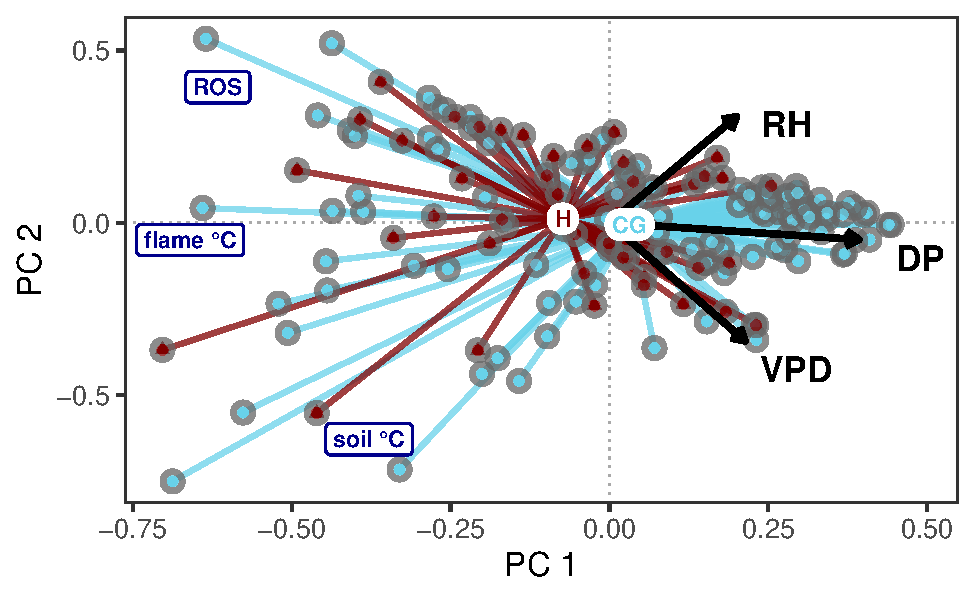
\includegraphics[width = 1\columnwidth]{pca_gg-1.pdf}
\caption{Principal Components Analysis of fire behavior data (response
variables in blue; rate of spread (ROS), temperature above surface
(flame \degC), and temperature at soil surface (soil \degC) for prescribed
burns on rangeland at Hettinger (H), in southwestern North Dakota, and
Central Grasslands (CG), in central North Dakota. No difference between
locations ($P$ = 0.11). 
Total variance explained in these two axes = 86\%.}
\label{PCA}
\end{figure}

Fires at both locations were characterized by considerable variability
among sub-plots. Above the soil surface, half of the fires (13) exceeded
325\(^\circ\)C, but only four of those fires had \textgreater50\% of
individual sample plots within the burns reach an average of
325\(^\circ\)C. Sparse fuels meant that fire did not spread to some
individual plots in some burns despite strip ignitions. Among plots that
burned, fewer than half exceeded 100\(^\circ\)C at the soil surface (49
of 121 plots). A majority of the fires (18) had at least one plot exceed
100\(^\circ\)C at the soil surface, seven had over half of the plots
exceed 100\(^\circ\)C at the soil surface, and only one fire had all
plots reach this (a spring Central Grasslands fire). Only 10 fires
reached or exceeded 325\(^\circ\)C on the soil surface, with most of
these fires reaching this point in only one plot and never in more than
half of the plots.

\begin{figure}
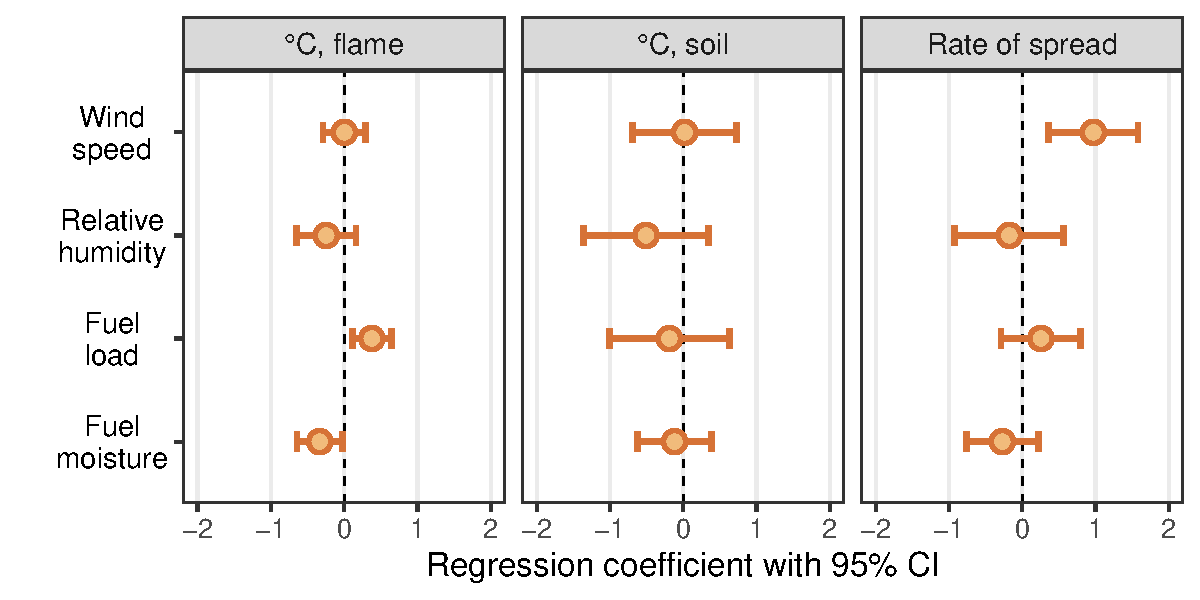
\includegraphics[width = 1\columnwidth]{CI_gg-1.pdf}
\caption{Regression coefficients and 95\% confidence intervals for fuel
and weather terms from models for maximum temperature at 15 cm above the
soil surface (flame), maximum temperature at the soil surface (soil),
and rate of spread.}
\label{CIs}
\end{figure}


The effects of fuel and fire weather predictor variables varied across the three response variables (Fig.~\ref{CIs}). 
Fires spread faster with higher wind speeds ($t$ = 2.92, $P~<$ 0.01), but no other variable had a statistically-significant association with rate of spread (Table~\ref{RegResults}).
Aboveground flame temperatures increased as fuel load increased $(t$ = 2.82, $P$ = 0.01) and decreased as fuel moisture increased ($t$ = -2.16, $P$ = 0.04). 
No fuel or weather variable included here had statistically-significant associations with soil surface temperature
(Table~\ref{RegResults}).

\begin{table}
\caption{Results of generalized linear mixed effect regression models testing three measure of fire behavior against four potential predictor variables. 
Statistics reflect pooled results of 50 imputed datasets using the \emph{mice} package in \textsf{R},  see Methods. Vapor pressure deficit
included for Rate of spread only due to statistically-significant
difference between GLMM regression results that included VPD compared to
RH alone (Wald = 5.32, $P$ = 0.02), while temperature models had no such
difference. \label{RegResults} }
\centering 
\begin{tabular}{llcc}
\toprule
Response & Model term & $t_{df}$ & P \\
\midrule

Rate of spread & & & \\
& Wind speed & $2.92_{108.0}$ & \textless{} 0.01 \\
& Vapor pressure deficit & -2.31 108.1 & 0.02 \\
& Relative humidity & -1.66 80.8 & 0.10 \\
& Fuel load & 1.16 49.9 & 0.25 \\
& Fuel moisture & -0.68 62.9 & 0.50 \\
Canopy temperature & & & \\
& Fuel load & 2.82 54.2 & 0.01 \\
& Fuel moisture & -2.16 40.9 & 0.04 \\
& Relative humidity & -1.19 120.4 & 0.24 \\
& Wind speed & 0.02 132.4 & 0.99 \\
Surface temperature & & & \\
& Relative humidity & -1.19 74.8 & 0.24 \\
& Fuel load & -0.48 20.1 & 0.64 \\
& Fuel moisture & -0.47 40.1 & 0.64 \\
& Wind speed & 0.06 49.5 & 0.95 \\
\bottomrule
\end{tabular}
\end{table}

\hypertarget{discussion}{%
\section{Discussion}\label{discussion}}

In our comparison of three measurements of fire behavior---rate of spread and maximum temperature recorded on the soil surface and 15 cm
above the soil surface---against fuel and fire weather variables, we
found considerable variability in which predictor variables were
associated with different measures of fire behavior. These data directly
support the safe and effective application of prescribed fire in the
region. Some results are straightforward and consistent with decades of
fire safety science; e.g., faster rates of fire spread are associated
with higher wind speed and lower relative humidity. Other results add
nuance to an ecological understanding of how fire behavior relates to
fire effects---e.g., factors like fuel load and overall fuelbed moisture
were related with flame temperature but not soil surface temperature,
which suggests that direct effects on belowground plant tissue and soil
biota are not correlated with aboveground heating and fire spread.

To our knowledge, this is the first study from the northern Great Plains
to scrutinize the factors that influence fire behavior, and the first to
combine reports of fire spread and temperature data from thermocouples.
Most published research on fire spread in the Great Plains is derived
from computer simulations
\citep{mcgranahan2013, overholt2014, yurkonis2019}. The few field
studies from the region mostly report temperature data from
thermocouples and rarely incorporate fuel and fire weather data into the
analysis; when such information is provided, it is typically included in
the study description, not as data. Given the high degree of variability
in the wildland fire environment, a mechanistic understanding of
grassland fire dynamics will require collect fuel, fire weather, and
fire behavior data in a spatially and temporally consistent manner to
facilitate statistical analyses of their relationships
\citep{hiers2020, mcgranahan2018}.

Mean temperatures recorded in this study are consistent with other
reports from northern rangelands. In central Alberta grassland,
\citet{bailey1980} observed that surface temperatures varied between
110\(^\circ\)C and 165\(^\circ\)C for backfires and headfires,
respectively, and headfires averaged 200\(^\circ\)C 15 cm above the
ground; temperatures generally tracked with fuel load. Surface fires
through jack pine barrens in Ontario had a similar range as ours
\citep[140-545\(^\circ\)C,][]{smith1966}. In our study, mean 15-cm
temperatures were 225\(^\circ\)C during spring burns in central North
Dakota and 250\(^\circ\)C during fall burns in southwestern North
Dakota; surface temperatures at both locations generally averaged just
above 100\(^\circ\)C (Fig. 1).

Discrepancies between our data and others from the region are consistent
with what would be expected when differences in the fire environment are
considered. For example, \citet{ohrtman2015} reported a wide range of
maximum temperatures at the soil surface---150-500\(^\circ\)C---that was
generally explained by variability in annual productivity and clipping
frequency, which altered fuel load. Our fires were also cooler than
those reported by \citet{archibold2003} in Saskatchewan: using the
mid-point of observations made at 10 cm and 20 cm as a comparison to our
15-cm values, spring fires reached 314\(^\circ\)C and fall fires reached
298\(^\circ\)C. But \citet{archibold2003} also reported substantially
lower fuel moisture in each season and they had approximately three
times the fuel load, likely due to an absence of grazing on the remnant
prairie. A previous study reported similar results---temperatures
approaching 500\(^\circ\)C when fuel loads averaged 2.8-4.5 t
ha\(^{\text{-}1}\) \citep{archibold1998}. With greater variability in
fuel load and fuel moisture, we might also expect to see these factors
have greater influence on aboveground flame temperatures. For example,
in Colorado, \citet{augustine2014} observed a strong linear relationship
between fuel load and temperatures ranging from 60-200\(^\circ\)C, but
their fuel load also ranged from 0.2 to 1.2 t ha\(^{\text{-}1}\).

Fires at both of our locations spread much more slowly than most reports
from other grasslands, due primarily to high fuelbed moisture content
and little opportunity for mitigation by wind or lower atmospheric
moisture (Fig. 1). Perhaps the most variability in fire spread was
reported by \citet{sneeuwjagt1977} from prescribed grass fires in
California and Washington, where rates of spread ranged from 0.2-61 m
min\(^{\text{-}1}\). From grassland fires in South Africa and Kansas,
USA, \citet{trollope2002} reported average spread rates of 24 and 32 m
min\(^{\text{-}1}\), respectively, for head fires and 0.12 and 0.14 m
min\(^{\text{-}1}\), respectively, for back fires. In a tallgrass
prairie in Texas, \citet{clements2019} recorded fire spreading between
72-150 m min\(^{\text{-}1}\) with the wind and 48 m min\(^{\text{-}1}\)
for flanking fires. Likewise, fires through cured grass fuelbeds in
Australia spread much more rapidly than we observed---up to 18-180 m
min\(^{\text{-}1}\) \citep{cheney1993, cheney1995, cruz2015}. Through
partially-cured stands, though, \citet{cruz2015} found spread rates
dropped to 3-44 m min\(^{\text{-}1}\), approaching our location averages
of 2.1 and 3.1 m min\(^{\text{-}1}\). Consistent with our finding that
only wind speed had a statistically-significant effect on increasing
rate of spread (Fig. 3), \citet{cheney1993} found that wind was by far
the most important variable to spread rate.

Interestingly, \citet{cheney1993} found that fires spread faster in
undisturbed pastures compared to those that had been cut, which they
attribute to differences in fuel structure (height, bulk density) rather
than fuel load. This might have implications for fire behavior in our
region, where invasive species like \emph{Poa pratensis} generally
increase aboveground plant biomass but do so by adding thick dense
litter at the soil surface, rather than standing dead fuel in the plant
canopy \citep{gasch2020}. While difficult to tease apart statistically
in the present data, many burn units in our mesic location in central
North Dakota were dominated by \emph{P. pratensis} and indeed, that
location tended to have higher fuel loads and lower rates of spread
(Fig.~\ref{DataSummary}), consistent with simulations of fire spread through those
\emph{P. pratensis}-dominated prairies \citep{yurkonis2019}.

Much is made of the difference in fire behavior between head and back
fires in the fire ecology literature, and while we expect these
differences translate to different fire effects in our system, making
distinctions between fire types is difficult in both our data and our
management. \citet{trollope1978} emphasized that while head fires move
faster and generally release more energy, back fires effect greater
heating at the ground level. One would expect, then, that back fires
would have more opportunity to burn down through even thick \emph{P.
pratensis} litter to mineral soil. Unfortunately, our results offer
little insight into what fuel or weather variables enhance litter
combustion, likely because most of our fires never got very hot at the
soil surface---50\% of our observations were less than 60\(^\circ\)C,
and 60\% less than 100\(^\circ\)C (Fig.~\ref{DataSummary}). 
Nor can we differentiate the direction of fire spread with the current trigonometry applied to the
triangular thermocouple arrays \citep{simard1984}, although it would
theoretically be possible to compare spread direction to wind direction
if the latter data were available at a fine enough scale.

The functional difference between head and back fires in the fuelbeds
reported here is likely moot. Because our fuels were often sparse,
sometimes only marginally cured, and prescriptions precluded taking
advantage of higher wind or lower relative humidity to mitigate fuel
limitations, we often employed substantial interior ignitions using
strip, point, flanking, and spiral patterns that sent flame fronts
towards our sensors in all possible directions at different times. While
\citet{williams2015} did show that different ignition patterns created
additional spatial variability in fire behavior, the effect of shorter
line ignitions and spot ignitions was to mitigate the high severity of
wildfire and long line ignitions in highly-flammable spinifex fuelbeds.
In our case, we had to manipulate ignition pattern just to get fire to
carry. Our data are certainly useful in describing the variability in
fire behavior across these burns, but do not inform the relationship
between ignition pattern and fire behavior. Thus, future research on
fire behavior in the northern Great Plains should (1) use experimental
plots with consistent fuelbeds to explicitly compare head and back fires
set via line ignitions, akin to the experimental burning program
described by \citet{cruz2015} in Australia, and (2) attempt to at least
address severity, if not fire behavior, in wildfire scenarios via remote
sensing and/or modelling.

A more detailed analysis of fuelbed effects on fire behavior also ought
to separate fuels into live and dead components, and consider the
moisture content of each along with fuel load ratios. Explicitly
measuring litter moisture might also be valuable, especially when
variability in belowground heating is expected to influence first-order
fire effects. We report here the overall fuel moisture content of the
entire fuelbed, consistent with descriptive, post hoc statistical
approaches to describing fire behavior
\citep{trollope1978, trollope1985, bidwell1992, trollope2002, mcgranahan2016}.
But predictive fire behavior models accommodate inputs for live and dead
fuel categories \citep{scott2005}, and \citet{kidnie2015a} found that
four categories of live, dead, and senescent fuels best represented
differences in grassland fuel moisture scenarios. With this in mind,
\citet{cruz2015} employed a hybrid approach in which fuel moisture was
measured for the various components, from which a weighted average was
used as a predictor variable in regression analysis. They subsequently
found that overall degree of curing, not simply live fuel moisture, was
the most important variable in explaining the dampening effect of fuel
moisture on fire behavior.

Often, time and resource constraints preclude the separation of fine
plant material by live and dead class, and overall fuelbed moisture
content is the best available data for managers. Although parsing live
and dead fuel moisture in the present analysis would probably not better
explain variability in our dataset, it would likely contribute to better
predictions of fire behavior relative to management objectives if
information on overall fuelbed moisture content were available prior to
ignition. Unfortunately, the standard clipping and drying method is not
compatible with providing day-of fuel moisture data, and visual
assessments based on color tend to over-predict curedness
\citep{kidnie2015a}. However, electronic devices can provide accurate
and instantaneous measurements of grassland fuel moisture
\citep{mcgranahan2019}.

Research must also address the influence of atmospheric moisture
conditions on prescribed fire behavior. Several broad-scale, post-hoc 
analyses of wildfire conditions conclude that atmospheric moisture is an
important driver of burned area \citep{evett2008, reid2010, sedano2014}.
But experiments that explicitly test the immediate effect of relative
humidity on fire behavior report no appreciable effect on surface fire
temperatures or rate of spread \citep{sparling1966, trollope1985}. It is
likely that atmospheric moisture plays a larger role in modulating fuel
moisture content prior to combustion than affecting instantaneous fire
behavior itself---consider how fire behavior models take fuel moisture
as a parameter and not relative humidity, but include relative humidity
as an input to determine fuel moisture content
\citep{rothermel1983, cruz2016}.

The most appropriate measure of atmospheric moisture content might also
be unresolved. We focused our analysis here on relative humidity because
it is so common in fire behavior models and fire weather forecasts. But
vapor pressure deficit has also been identified as an important driver
of fire spread and intensity \citep{gomes2020}. In fact,
\citet{srock2018} suggest vapor pressure deficit might be a better
measure of atmospheric moisture content for fire predictions, but the
Hot-Dry-Windy index they developed to incorporate vapor pressure deficit
operates at synoptic scales beyond the spatial extent and operational
periods of prescribed burns. Given that substantial changes in
atmospheric moisture changes in recent decades are expected to
strengthen over the 21\textsuperscript{st} century
\citep{seager2015, ficklin2017}, understanding how these dynamics affect
fire behavior will be an essential component of managing resilient fire
regimes.

This study is novel in that it examines the fire environment at a spatial scale consistent with land management in the region using
realistic ignition scenarios. 
To our knowledge, no other study in the northern Great Plains has reported the behavior of fires larger than experimental plots. Integrating research into management almost invariably requires trade-offs; two already discussed above include (1)
measuring only the overall moisture content of the entire fuelbed, being
precluded from parsing fuel into live, dead, and litter components, and
(2) measuring two-dimensional rate of spread of fire fronts within the
burn unit without being able to associate them with wind direction. But
these are the respective conditions under which prescribed fire managers
in the region decide whether to burn, and ensure fire spread objectives
are met. Research conducted at the spatial scales at which management
occurs helps managers trust the transfer of knowledge from studies to
working landscapes \citep{sayre2005, cacciapaglia2012}. For example, all
of our fire behavior measurements were made more than 50 m from the
initial fire line, the distance identified in simulations and used in
wildland fire science to allow flame fronts to achieve a quasi-steady
state in spread rate \citep{fernandes2000, sutherland2020}, which is
obviously precluded in studies that employ small plots.

\backmatter

\bmhead{Supplementary Information}

Supplementary Information containing additional information on the study location, rate of spread calculations, and \textsf{R} script is available in the online version of the paper.

\bmhead{Acknowledgments}

We appreciate support from the North Dakota State Agricultural Experiment Station, including K. Sedivec at the Central Grasslands REC and C. Schauer and B. Geaumont at the Hettinger REC. 
We recognize funding from the University of North Dakota Department of Biology, USDA-NIFA Hatch project number ND02393, and USDA-NIFA AFRI award number 2018-67020-27856. 
We appreciate the technical assistance of several North Dakota State University graduate students and faculty for assistance with prescribed burning. 
L. LaFond, C. LaFond, and E. Wahl assisted with datalogger assembly. J. Spiess, J. Cutter, M. Lakey, B. Poling, and A. Steele assisted with sensor deployment and data collection.

 \bibliography{FireBehaviorBib.bib}

\end{linenumbers}
\end{document}
